%%%%%%%%%%%%%%%%%%%%%%%%%%%%%%%%%%%%%%%%%%%%%%%%%%%%%%%%%%%%%%%%%%%%%%%%%%%%%%%%
\section{Android User Interface}
%%%%%%%%%%%%%%%%%%%%%%%%%%%%%%%%%%%%%%%%%%%%%%%%%%%%%%%%%%%%%%%%%%%%%%%%%%%%%%%%
%------------------------------------------------------------------------------
\begin{frame}
\frametitle{Android User Interface}
\begin{columns}
 \column{0.33 \textwidth}
	\begin{figure}
	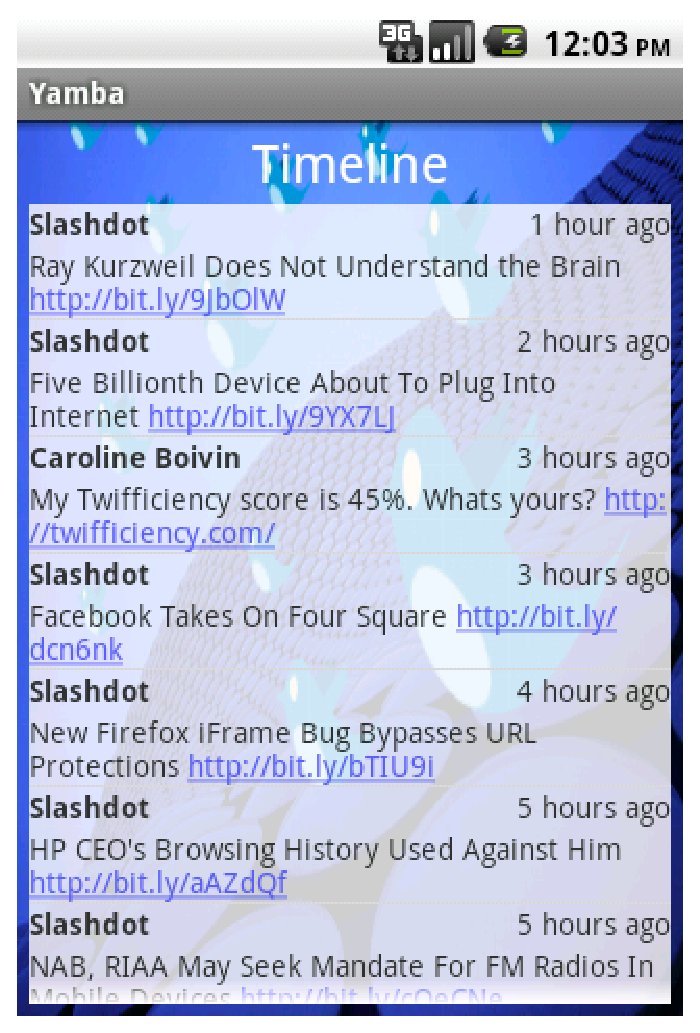
\includegraphics[width= 0.8 \textwidth]{fig-30.eps}
	\caption{List of status messages from other people, called a timeline}
	\end{figure}
 \column{0.33 \textwidth}
	\begin{figure}
	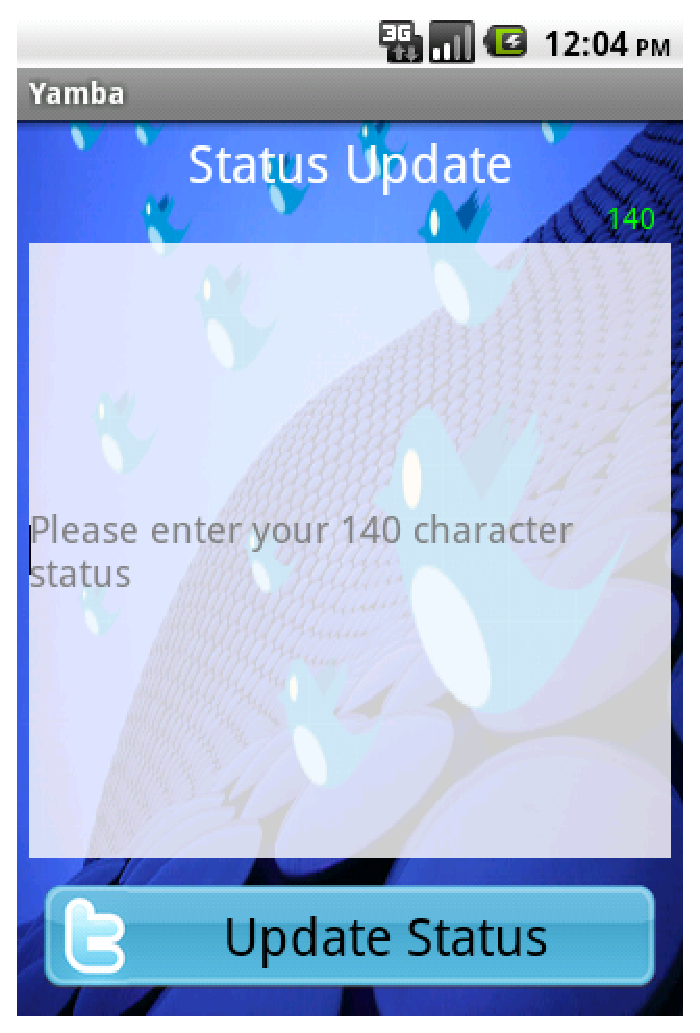
\includegraphics[width= 0.8 \textwidth]{fig-31.eps}
	\caption{Screen where the user can enter a status message}
	\end{figure}
 \column{0.34 \textwidth}
	\begin{figure}
	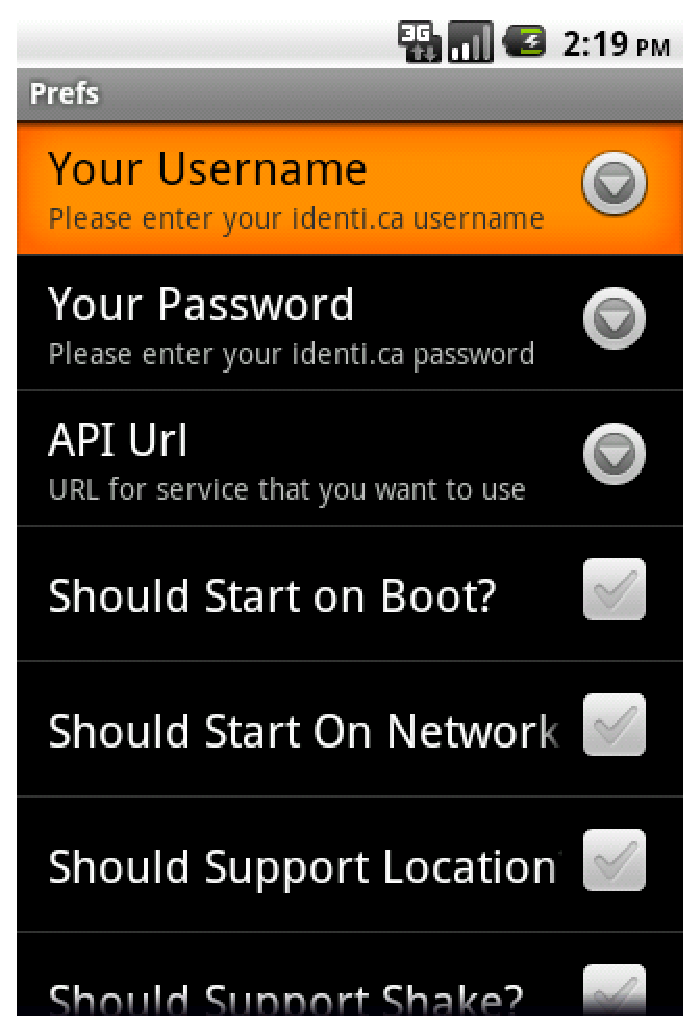
\includegraphics[width= 0.8 \textwidth]{fig-32.eps}
	\caption{User preferences}
	\end{figure}
\end{columns}

\end{frame}

%------------------------------------------------------------------------------
\subsection{Starting the Yamba Project}
\begin{frame}
\frametitle{Starting the Yamba Project}
File|New Android Application Project\\
\begin{columns}
\column{0.5 \textwidth}
	\begin{figure}
	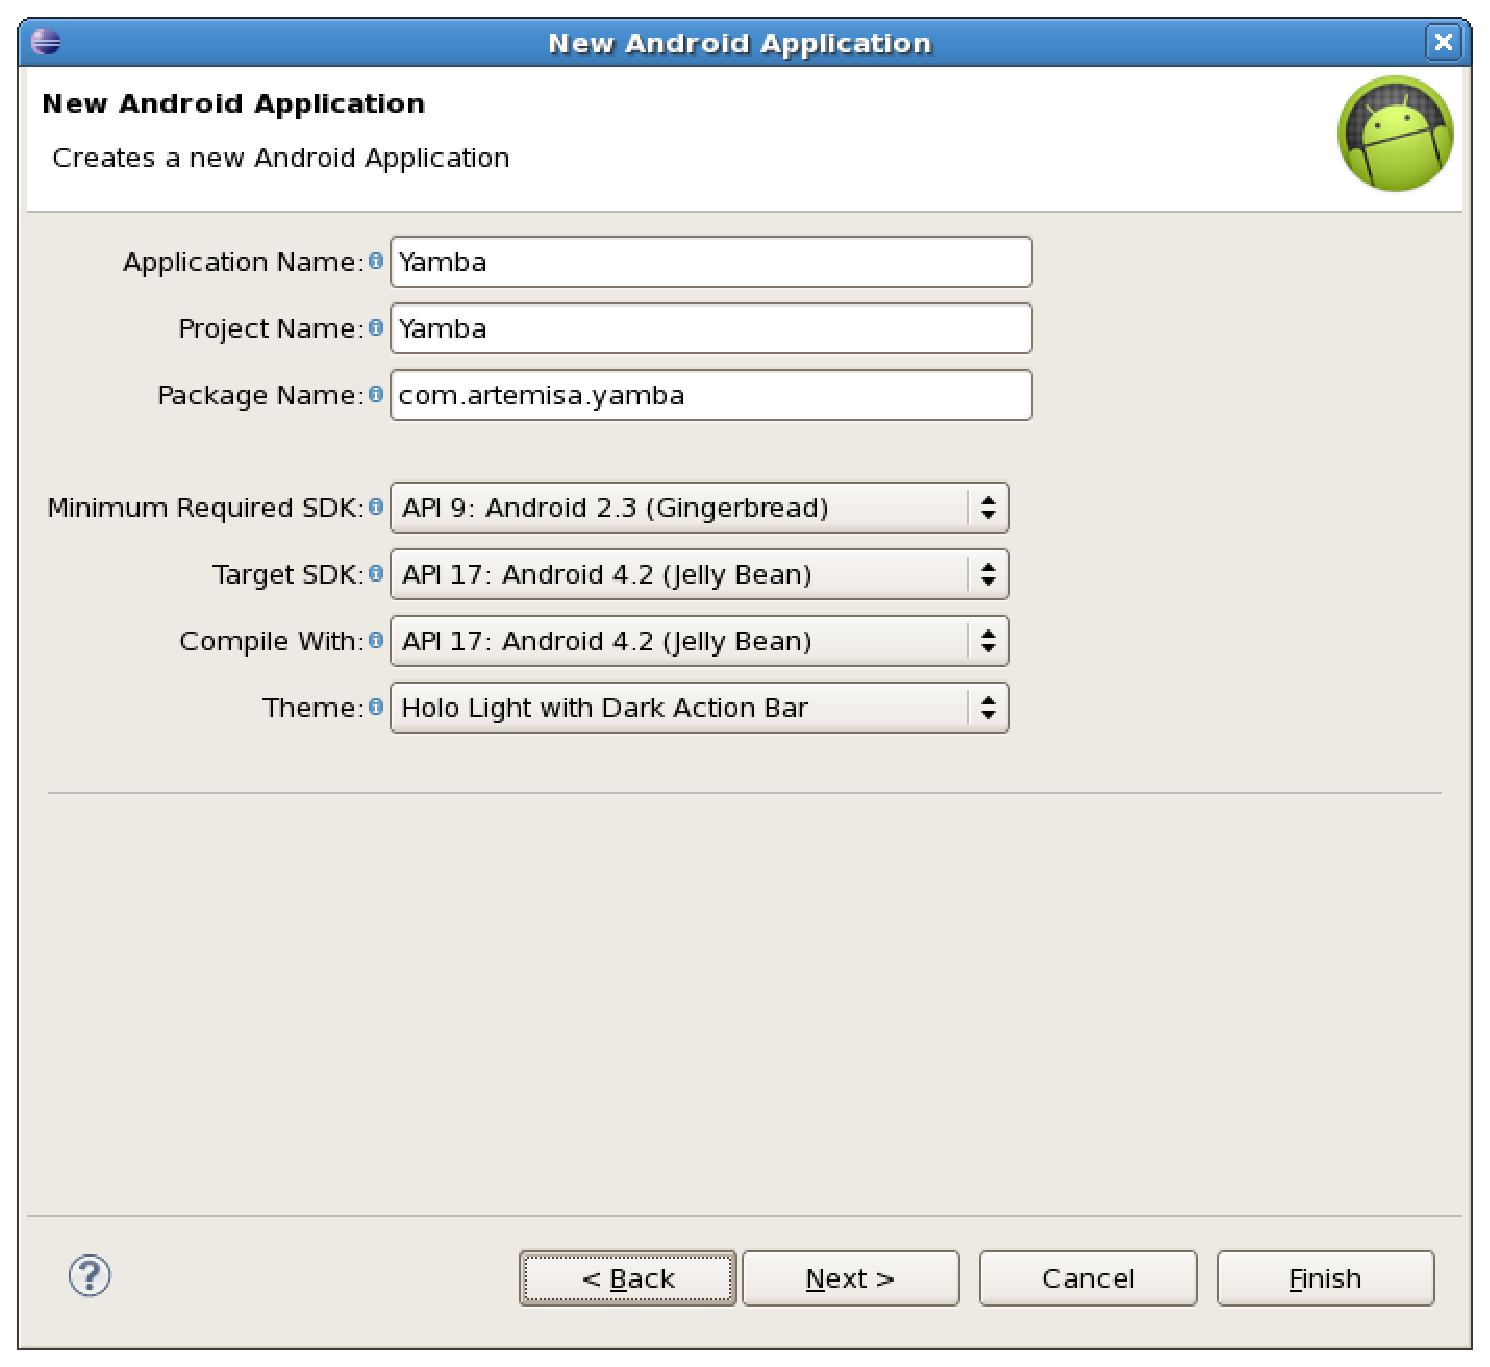
\includegraphics[width= 0.8 \textwidth]{yambaNewAndroidApplication1.eps}
	\caption{Application Name \texttt{Yamba}, Project Name \texttt{Yamba} and Package Name \texttt{com/artemisa/yamba}}
	\end{figure}
 \column{0.5 \textwidth}
	\begin{figure}
	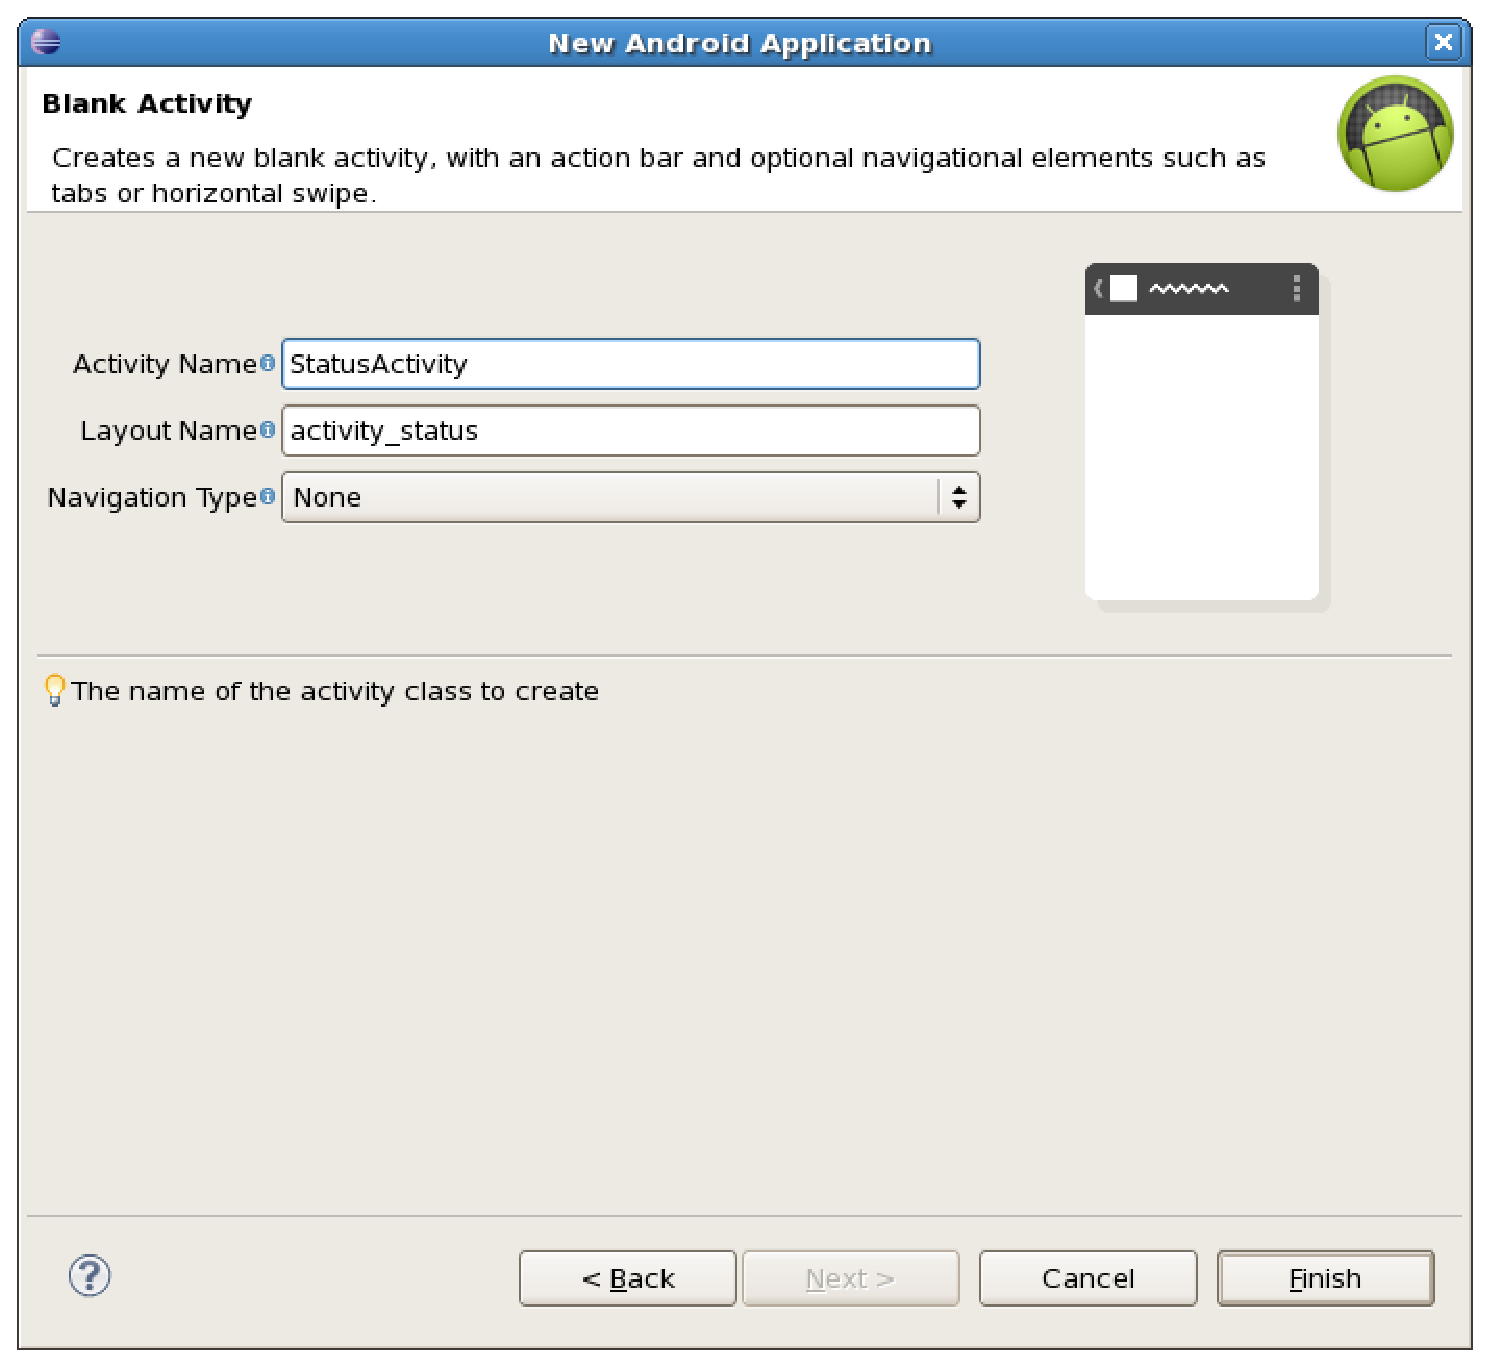
\includegraphics[width= 0.8 \textwidth]{yambaNewAndroidApplication2.eps}
	\caption{Activity Name \texttt{StatusActivity} and Layout Name \texttt{activity\_status}}
	\end{figure}
\end{columns}
\end{frame}
%------------------------------------------------------------------------------
\subsection{Git}
\begin{frame}
\frametitle{Git}
\begin{enumerate}
\item Fisrt Time System Setup
	\begin{enumerate}
 		\item \texttt{git config --global user.name "Juan García"}
 		\item \texttt{git config --global user.email juangarcia@mailinator.com}
	\end{enumerate}
\item First Time Repository Setup
	\begin{enumerate}
		\item Define \texttt{.gitignore}
		\item \texttt{git init}
	\end{enumerate}
\item Adding and Committing
	\begin{enumerate}
		\item \texttt{git add .}
		\item \texttt{git status}
		\item \texttt{git commit -m  ``Initial commit''}
	\end{enumerate}

\end{enumerate}
\end{frame}
%------------------------------------------------------------------------------
\subsection{The StatusActivity Layout}
\begin{frame}
\frametitle{The StatusActivity Layout}
\begin{columns}
 \column{0.65 \textwidth}
This screen will have four components
\begin{enumerate}
	\item A title at the top of the screen. \texttt{TextView} widget
	\item A big text area to type our 140-character status update. \texttt{EditText} widget
	\item A button to click to update the status. \texttt{Button} widget
	\item A layout to contain all these widgets and lay them out one after another in a vertical fashion. \texttt{LinearLayout}
\end{enumerate}
\column{0.35 \textwidth}
	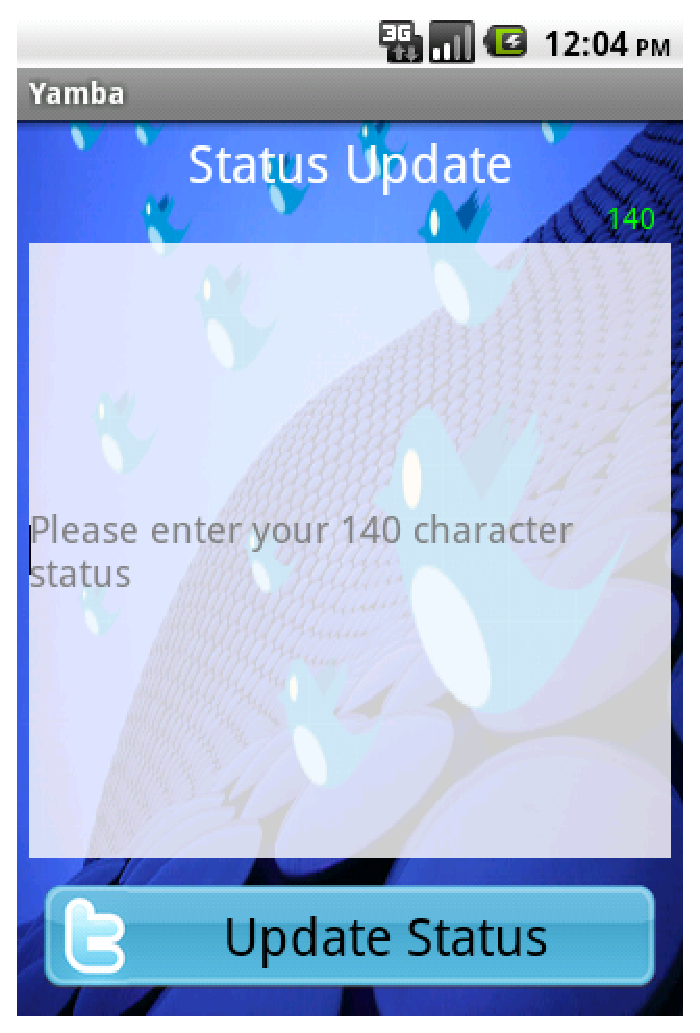
\includegraphics[width= 0.8 \textwidth]{fig-31.eps}
\end{columns}

\end{frame}
%------------------------------------------------------------------------------
\begin{frame}[allowframebreaks,containsverbatim]
\frametitle{Layout XML Code}
This code was generated by Eclipse Graphical Layout
\lstset{language=XML, style=eclipse}
%\begin{adjustbox}{width=1.0 \textwidth}
\begin{lstlisting}[caption=res/layout/activity\_status.xml, basicstyle=\scriptsize,escapechar=!]
<LinearLayout xmlns:android="http://schemas.android.com/apk/res/android"
    xmlns:tools="http://schemas.android.com/tools"
    android:id="@+id/LinearLayout"
    !\colorbox{light-gray}{android:layout\_width="fill\_parent"}!
    !\colorbox{light-gray}{android:layout\_height="fill\_parent"}!
    !\colorbox{light-gray}{android:orientation="vertical"}!
    android:paddingBottom="@dimen/activity_vertical_margin"
    android:paddingLeft="@dimen/activity_horizontal_margin"
    android:paddingRight="@dimen/activity_horizontal_margin"
    android:paddingTop="@dimen/activity_vertical_margin"
    tools:context=".StatusActivity" > !\pagebreak!

    <TextView
        !\colorbox{light-gray}{android:layout\_width="fill\_parent"}!
        !\colorbox{light-gray}{android:layout\_height="wrap\_content"}!
        !\colorbox{light-gray}{android:layout\_margin="10dp"}!
        !\colorbox{light-gray}{android:gravity="center"}!
        !\colorbox{light-gray}{android:text="@string/titleStatus"}!
        !\colorbox{light-gray}{android:textSize="30sp"}! /> !\pagebreak!

    <EditText
        android:id="@+id/editText"
        !\colorbox{light-gray}{android:layout\_width="fill\_parent"}!
        !\colorbox{light-gray}{android:layout\_height="fill\_parent"}!
        !\colorbox{light-gray}{android:layout\_weight="1"}!
        android:ems="10"
        !\colorbox{light-gray}{android:gravity="top|left"}!
        !\colorbox{light-gray}{android:hint="@string/hintText"}! >
        <requestFocus />
    </EditText> !\pagebreak!

    <Button
        !\colorbox{light-gray}{android:id="@+id/buttonUpdate"}!
        !\colorbox{light-gray}{android:layout\_width="fill\_parent"}!
        !\colorbox{light-gray}{android:layout\_height="wrap\_content"}!
        !\colorbox{light-gray}{android:text="@string/buttonUpdate"}!
        !\colorbox{light-gray}{android:textSize="20sp"}! />

</LinearLayout>
\end{lstlisting}
%\end{adjustbox}
\end{frame}
%------------------------------------------------------------------------------
\begin{frame}
\frametitle{Important Widget Properties}
\begin{description}
	\item[\texttt{layout\_height} and \texttt{layout\_width}] Defines how much space this widget is asking from its parent layout to display
itself. Best practice would be to use either \texttt{fill\_parent} or \texttt{wrap\_content} for the value
	\item[\texttt{layout\_gravity}]Specifies how this particular widget is positioned within its layout, both horizontally
and vertically. \texttt{top}, \texttt{center}, \texttt{left} \dots
	\item[\texttt{gravity}] Specifies how the content of this widget is positioned within the widget itself
	\item[\texttt{text}] It simply specifies the text for the widget
	\item[\texttt{id}] \texttt{id} is simply the unique identifier for this particular widget in a particular layout resource file
\end{description}
\end{frame}
%------------------------------------------------------------------------------
\begin{frame}[fragile]
\frametitle{Strings Resource}
\lstset{language=XML, style=eclipse}
\begin{adjustbox}{width=1.0 \textwidth}
\centering
\begin{lstlisting}[caption=res/values/strings.xml]
<?xml version="1.0" encoding="utf-8"?>
<resources>
    <string name="app_name">Yamba</string>
    <string name="action_settings">Settings</string>
    <string name="hello_world">Hello world!</string>
    <string name="titleStatus">Status Update</string>

    <string name="hintText">Please entrer your 140-character status</string>

    <string name="buttonUpdate">Update</string>
</resources>
\end{lstlisting}
\end{adjustbox}
\end{frame}


%------------------------------------------------------------------------------
\begin{frame}[fragile]
\frametitle{Observer Pattern}
\url{http://en.wikipedia.org/wiki/Observer_pattern}\\
\begin{columns}
\column{1.0 \textwidth}
	\begin{figure}
	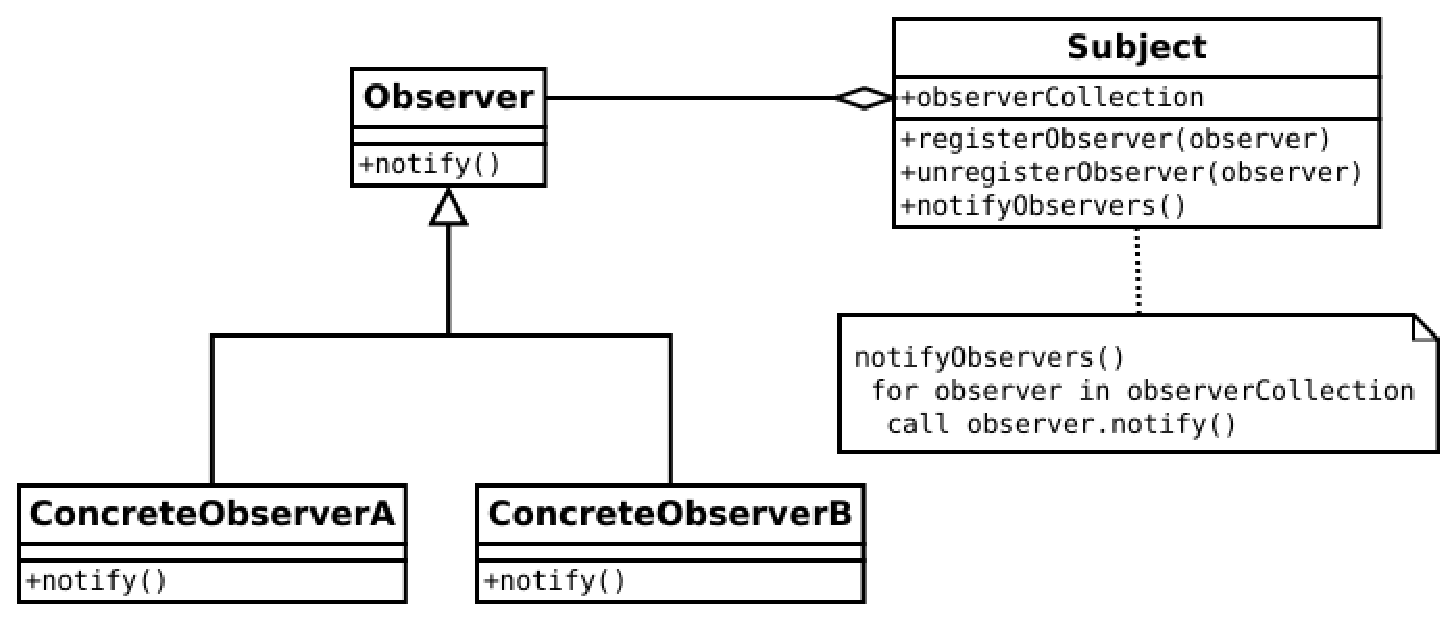
\includegraphics[width= 1.0 \textwidth]{observer.eps}
	\caption{UML class diagram of Observer pattern}
	\end{figure}
\end{columns}
\end{frame}
%------------------------------------------------------------------------------
\begin{frame}[allowframebreaks,containsverbatim]
\frametitle{The StatusActivity Java Class}
\lstset{language=java, style=eclipse, breaklines=true, tabsize=2}
%\begin{adjustbox}{width=1.0 \textwidth}
\centering
\begin{lstlisting}[caption=src/com/artemisa/yamba/StatusActivity.java, basicstyle=\tiny, escapechar=! ]
// .
// .
// .
public class StatusActivity extends Activity implements OnClickListener { // !\circled{1}!

	private static final String TAG = "Status Activity";
	private Button updateButton;
	private EditText editText;

	@Override
	protected void onCreate(Bundle savedInstanceState) {
		super.onCreate(savedInstanceState);
		setContentView(R.layout.activity_status);

		// Find views and set Observer !\circled{2}!
		updateButton = (Button) findViewById(R.id.buttonUpdate);
		updateButton.setOnClickListener(this);

		editText = (EditText) findViewById(R.id.editText);
	}

	@Override
	public boolean onCreateOptionsMenu(Menu menu) {
		// Inflate the menu; this adds items to the action bar if it is present.
		getMenuInflater().inflate(R.menu.status, menu);
		return true;
	}

	// Called whe button is clicked !\circled{3}!
	public void onClick(View v) {
		Log.d(TAG, "OnClic:" + editText.getText().toString());
	}

}

\end{lstlisting}
%\end{adjustbox}
\end{frame}
%------------------------------------------------------------------------------
\begin{frame}[fragile]
\frametitle{Git}
\begin{enumerate}
\item \texttt{git status}
\item \texttt{git commit -a -m ``OnClickListener''}

\end{enumerate}


\end{frame}
%------------------------------------------------------------------------------
\subsection{Connecting on Twitter}

\begin{frame}[fragile]
\frametitle{Connecting on Twitter}
\url{http://yamba.maracana.com}

To make our life with web services and the Twitter API easier, we’re going to use a
third-party library, \href{http://www.winterwell.com/software/jtwitter.php}{jtwitter.jar}, provided by Winterwell Associates

\begin{itemize}
 \item Once you download this library, you can put it inside your project in Eclipse. Copy \texttt{jtwitter-yamba.jar} in \texttt{libs} directory
 \item Add \texttt{jtwitter-yamba.jar} to the \alert{classpath}, right-click on your project, select Properties, and you will get a Properties for Yamba
dialog window. Select Java Build Path, and choose the Libraries tab. In there, click on Add External JARs… and locate your jtwitter.jar file

\end{itemize}

\end{frame}
%------------------------------------------------------------------------------
\begin{frame}[fragile]
\frametitle{Updating the Manifest File for Internet Permission}
\lstset{language=XML, style=eclipse}
\begin{adjustbox}{width=0.75 \textwidth}
\centering
\begin{lstlisting}[caption=AndroidManifest.xml,basicstyle=\tiny, escapechar=$]
<?xml version="1.0" encoding="utf-8"?>
<manifest xmlns:android="http://schemas.android.com/apk/res/android"
    package="com/artemisa/yamba1"
    android:versionCode="1"
    android:versionName="1.0" >

    <uses-sdk
        android:minSdkVersion="8"
        android:targetSdkVersion="17" />
    <uses-permission android:name="android.permission.INTERNET" /> <!-- $\circled{1}$ -->
	
    <application
        android:allowBackup="true"
        android:icon="@drawable/ic_launcher"
        android:label="@string/app_name"
        android:theme="@style/AppTheme" >
        <activity
            android:name="com/artemisa/yamba1.StatusActivity"
            android:label="@string/app_name" >
            <intent-filter>
                <action android:name="android.intent.action.MAIN" />

                <category android:name="android.intent.category.LAUNCHER" />
            </intent-filter>
        </activity>
    </application>

</manifest>
\end{lstlisting}
\end{adjustbox}
\end{frame}
%------------------------------------------------------------------------------

\begin{frame}[allowframebreaks,containsverbatim]
\frametitle{The StatusActivity Java Class}
\lstset{language=java, style=eclipse, breaklines=true, tabsize=2}
%\begin{adjustbox}{width=1.0 \textwidth}
\centering
\begin{lstlisting}[caption=src/com/artemisa/yamba/StatusActivity.java, basicstyle=\tiny, escapechar=!, ]
// .
// .
// .
public class StatusActivity extends Activity implements OnClickListener {
	private static final String TAG = "StatusActivity";
	private Button updateButton;
	private EditText editText;
	private Twitter twitter; // !\circled{1}!

	@Override
	protected void onCreate(Bundle savedInstanceState) {
		super.onCreate(savedInstanceState);
		setContentView(R.layout.activity_status);
	
		// Find views
		updateButton = (Button) findViewById(R.id.buttonUpdate);
		updateButton.setOnClickListener(this);
	
		editText = (EditText) findViewById(R.id.editText);
	
		twitter = new Twitter("student", "password"); // !\circled{2}!
		twitter.setAPIRootUrl("http://yamba.marakana.com/api");
	}

	@Override
	public boolean onCreateOptionsMenu(Menu menu) {
		// Inflate the menu; this adds items to the action bar if it is present.
		getMenuInflater().inflate(R.menu.status, menu);
		return true;
	}

	// Called when button is clicked
	public void onClick(View v) { // !\circled{4}!
		try {
			twitter.setStatus(editText.getText().toString());
			Log.d(TAG, "OnCLick: " + editText.getText().toString());
		} catch (TwitterException e) {
			Log.e(TAG, e.toString());
			e.printStackTrace();
		}
	}

}

\end{lstlisting}
%\end{adjustbox}
\end{frame}

%------------------------------------------------------------------------------

\begin{frame}[fragile]
\frametitle{Git}
\begin{enumerate}
\item \texttt{git status}
\item \texttt{git commit -a -m ``Connecting on Twitter''}

\end{enumerate}

\end{frame}
%------------------------------------------------------------------------------
\subsection{Toast}

\begin{frame}[fragile]
\frametitle{Toast}

\lstset{language=java, style=eclipse, breaklines=true, tabsize=2}
A toast provides simple feedback about an operation in a small popup. It only fills the amount of space required for the message and the current activity remains visible and interactive. 
\begin{lstlisting}
Context context = getApplicationContext();
CharSequence text = "Hello toast!";
int duration = Toast.LENGTH_SHORT;

Toast toast = Toast.makeText(context, text, duration);
toast.show();
\end{lstlisting}
\end{frame}
%------------------------------------------------------------------------------



\subsection{Asynchronous Threads}
\begin{frame}[fragile]
\frametitle{Asynchronous Task }

\lstset{language=java, style=eclipse, breaklines=true, tabsize=2}
\centering
\lstinline{private class MyTask extends AsyncTask<Params, Progress, Result> }

\begin{itemize}
\item An asynchronous task is defined by 3 generic types: \lstinline{Params}, \lstinline{Progress}, \lstinline{Result}

\item And 4 steps:
\lstinline{void onPreExecute()}, \lstinline{Result doInBackground(Params...)}, \lstinline{void onProgressUpdate(Progress...)}, \lstinline{void onPostExecute(Result)}

\item The task instance must be created on the UI thread. \lstinline{execute(Params...)} must be invoked on the UI thread

\item We need to create a new inner subclass \lstinline{PostToTwitter} of \lstinline{AsyncTask} and implement all methods. The \lstinline{PostToTwitter} class in this case will be an inner class of \lstinline{StatusActivity}

\end{itemize}

\end{frame}

%------------------------------------------------------------------------------



\begin{frame}[allowframebreaks,containsverbatim]
\frametitle{The StatusActivity Java Class}
\lstset{language=java, style=eclipse, breaklines=true, tabsize=2}
\begin{lstlisting}[caption=src/com/artemisa/yamba/StatusActivity.java, basicstyle=\tiny, escapechar=! ]
// .
// .
// .
public class StatusActivity extends Activity implements OnClickListener {
	// .
	// .
	// .
	// Asynchronously posts to twitter
	class PostToTwitter extends AsyncTask<String, Integer, String> { !\circled{1}!
		// Called to initiate the background activity
		@Override
		protected String doInBackground(String... statuses) { !\circled{2}!
			try {
				Twitter.Status status = twitter.updateStatus(statuses[0]);
				return status.text;
			} catch (TwitterException e) {
				Log.e(TAG, e.toString());
				e.printStackTrace();
				return "Failed to post";
			}
		} !\linebreak!

		// Called when there's a status to be updated
		@Override
		protected void onProgressUpdate(Integer... values) { !\circled{3}!
			super.onProgressUpdate(values);
			// Not used in this case
		}

		// Called when the background activity has completed
		@Override
		protected void onPostExecute(String result) { !\circled{4}!
			Toast.makeText(getApplicationContext(), result, Toast.LENGTH_SHORT)
					.show();
		} !\linebreak!
	}

	// Called when button is clicked
	public void onClick(View v) { !\circled{5}!
		String status = editText.getText().toString();
		new PostToTwitter().execute(status);
	} 

}
\end{lstlisting}
\end{frame}
%------------------------------------------------------------------------------
\begin{frame}[fragile]
\frametitle{Git}
\begin{enumerate}
\item \texttt{git status}
\item \texttt{git commit -a -m ``Asynchronous Threads''}
\end{enumerate}

\end{frame}
%------------------------------------------------------------------------------






\subsection{Other UI Events}
%------------------------------------------------------------------------------
\begin{frame}[fragile]
\centering
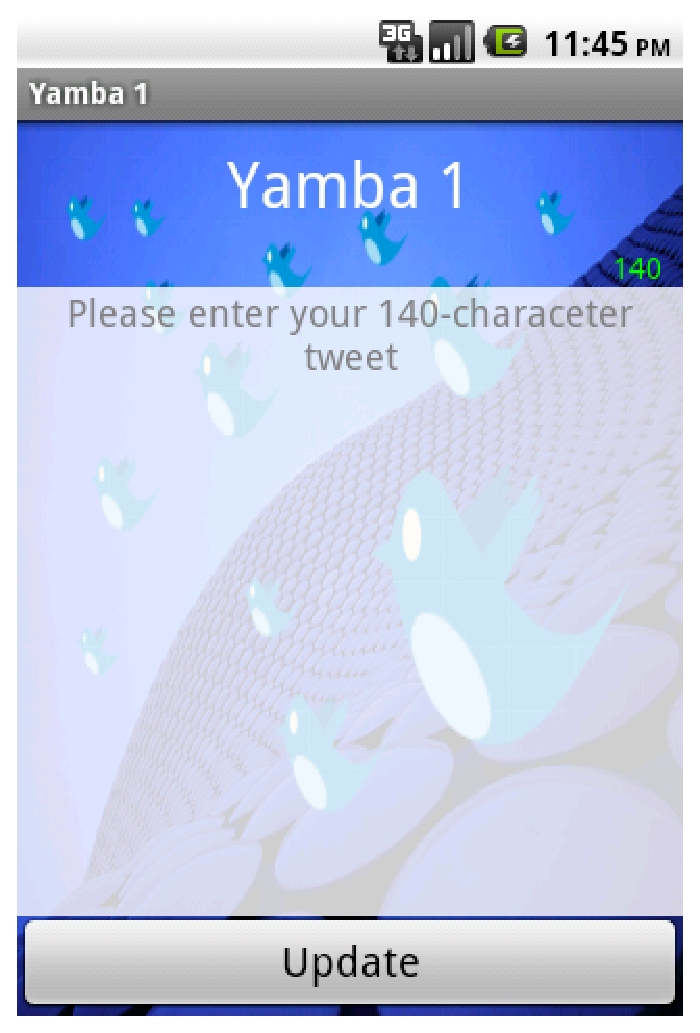
\includegraphics[width=0.4 \textwidth]{fig-063.eps}

\end{frame}
%------------------------------------------------------------------------------
\begin{frame}[allowframebreaks,containsverbatim]
\frametitle{activity\_status.xml}
\begin{itemize}
\item We’ll add another \texttt{TextView} to our layout to indicate how
many characters are still available. This text will change color, from green to yellow to
red
\lstset{language=XML, style=eclipse}
\begin{adjustbox}{width=0.8 \textwidth}
\begin{lstlisting}[caption=activity\_status.xml, escapechar=!]
<TextView
        android:id="@+id/textCount"
        android:layout_width="wrap_content"
        android:layout_height="wrap_content"
        android:layout_gravity="right"
        android:layout_marginRight="10dp"
        android:text="000" />
\end{lstlisting}
\end{adjustbox}
\end{itemize}

\end{frame}
%------------------------------------------------------------------------------
\begin{frame}[containsverbatim]
\frametitle{TextWatcher Interface}
\begin{itemize}
\item \texttt{TextWatcher} interface to watch for text changes

\end{itemize}

\lstset{language=java, style=eclipse, breaklines=true, tabsize=2, basicstyle=\footnotesize , numbers=none}
\begin{lstlisting}
void afterTextChanged(Editable s)
void beforeTextChanged(CharSequence s, int start, int count, int after)
void onTextChanged(CharSequence s, int start, int before, int count)
\end{lstlisting}
\end{frame}
%------------------------------------------------------------------------------
%------------------------------------------------------------------------------
\begin{frame}[allowframebreaks,containsverbatim]
\frametitle{The StatusActivity Java Class}
\lstset{language=java, style=eclipse, breaklines=true, tabsize=2}
\begin{lstlisting}[caption=src/com/artemisa/yamba/StatusActivity.java, basicstyle=\tiny, escapechar=! ]
// .
// .
// .
public class StatusActivity extends Activity implements OnClickListener,
		TextWatcher { // !\circled{1}!
	private static final String TAG = "StatusActivity";
	private Button updateButton;
	private EditText editText; 
	private Twitter twitter;
	private TextView textCount; // !\circled{2}!

	@Override
	protected void onCreate(Bundle savedInstanceState) {
		super.onCreate(savedInstanceState);
		setContentView(R.layout.activity_status);

		// Find views
		updateButton = (Button) findViewById(R.id.buttonUpdate);
		updateButton.setOnClickListener(this);

		editText = (EditText) findViewById(R.id.editText);
		editText.addTextChangedListener(this); // !\circled{3}! 

		textCount = (TextView) findViewById(R.id.textCount); // !\circled{4}!
		textCount.setText(Integer.toString(140)); 
		textCount.setTextColor(Color.GREEN);

		twitter = new Twitter("student", "password");
		twitter.setAPIRootUrl("http://yamba.marakana.com/api");
	}

	@Override
	public boolean onCreateOptionsMenu(Menu menu) {
		// Inflate the menu; this adds items to the action bar if it is present.
		getMenuInflater().inflate(R.menu.status, menu);
		return true;
	}
	
	// Asynchronously posts to twitter
	// .
	// .
	// .
	
	// Called when button is clicked
	public void onClick(View v) {
		String status = editText.getText().toString();
		new PostToTwitter().execute(status);
	}

	// Called when editText's text changes
	@Override
	public void afterTextChanged(Editable s) { // !\circled{5}!
		Log.d(TAG, "afterTextChanged()");

		int count = 140 - s.length();
		String text = Integer.toString(count);

		textCount.setText(text);

		if (count > 10) {
			textCount.setTextColor(Color.GREEN);
		} else {
			if (count >= 1 && count <= 10) {
				textCount.setTextColor(Color.YELLOW);
			} else {
				textCount.setTextColor(Color.RED);
			}
		}
	}

	
	@Override
	public void beforeTextChanged(CharSequence s, int start, int count,
			int after) {
		// not used
	}

	@Override
	public void onTextChanged(CharSequence s, int start, int before, int count) {
		// no used
	}
}

\end{lstlisting}
\end{frame}
%------------------------------------------------------------------------------

\begin{frame}[fragile]
\frametitle{Git}
\begin{enumerate}
\item \texttt{git status}
\item \texttt{git commit -a -m ``Other UI Events''}
\end{enumerate}

\end{frame}

%------------------------------------------------------------------------------
\subsection{Color and Graphics}
\begin{frame}[allowframebreaks,containsverbatim]
\frametitle{Color and Graphics}
\begin{itemize}
\item Create another drawable folder called simply \texttt{/res/drawable}
\item Add \texttt{background.png}
\end{itemize}

\lstset{language=XML, style=eclipse}
\begin{lstlisting}[caption=res/layout/activity\_status.xml, basicstyle=\scriptsize,escapechar=$]
<LinearLayout xmlns:android="http://schemas.android.com/apk/res/android"
    xmlns:tools="http://schemas.android.com/tools"
    android:id="@+id/LinearLayout"
    android:layout_width="fill_parent"
    android:layout_height="fill_parent"
    android:background="@drawable/background" <!-- $\circled{1}$ -->
    android:orientation="vertical"
    android:paddingBottom="@dimen/activity_vertical_margin"
    android:paddingLeft="@dimen/activity_horizontal_margin"
    android:paddingRight="@dimen/activity_horizontal_margin"
    android:paddingTop="@dimen/activity_vertical_margin"
    tools:context=".StatusActivity" > $\pagebreak$

    <TextView
        android:layout_width="fill_parent"
        android:layout_height="wrap_content"
        android:layout_margin="10dp"
        android:background="@android:color/white" <!-- $\circled{2}$ -->
        android:gravity="center"
        android:text="@string/titleStatus"
        android:textSize="30sp" />

    <TextView
        android:id="@+id/textCount"
        android:layout_width="wrap_content"
        android:layout_height="wrap_content"
        android:layout_gravity="right"
        android:layout_marginRight="10dp"
        android:text="000" /> $\pagebreak$
	
    <EditText
        android:id="@+id/editText"
        android:layout_width="fill_parent"
        android:layout_height="fill_parent"
        android:layout_weight="1"
        android:background="#cfff" <!-- $\circled{3}$ -->
        android:ems="10"
        android:gravity="top|center_horizontal"
        android:hint="@string/hintText" >

        <requestFocus />
    </EditText> $\pagebreak$

    <Button
        android:id="@+id/buttonUpdate"
        android:layout_width="fill_parent"
        android:layout_height="wrap_content"
        android:text="@string/buttonUpdate"
        android:textSize="20sp" />

</LinearLayout>
\end{lstlisting}
\end{frame}
%------------------------------------------------------------------------------
\begin{frame}
\frametitle{Summary}
\centering
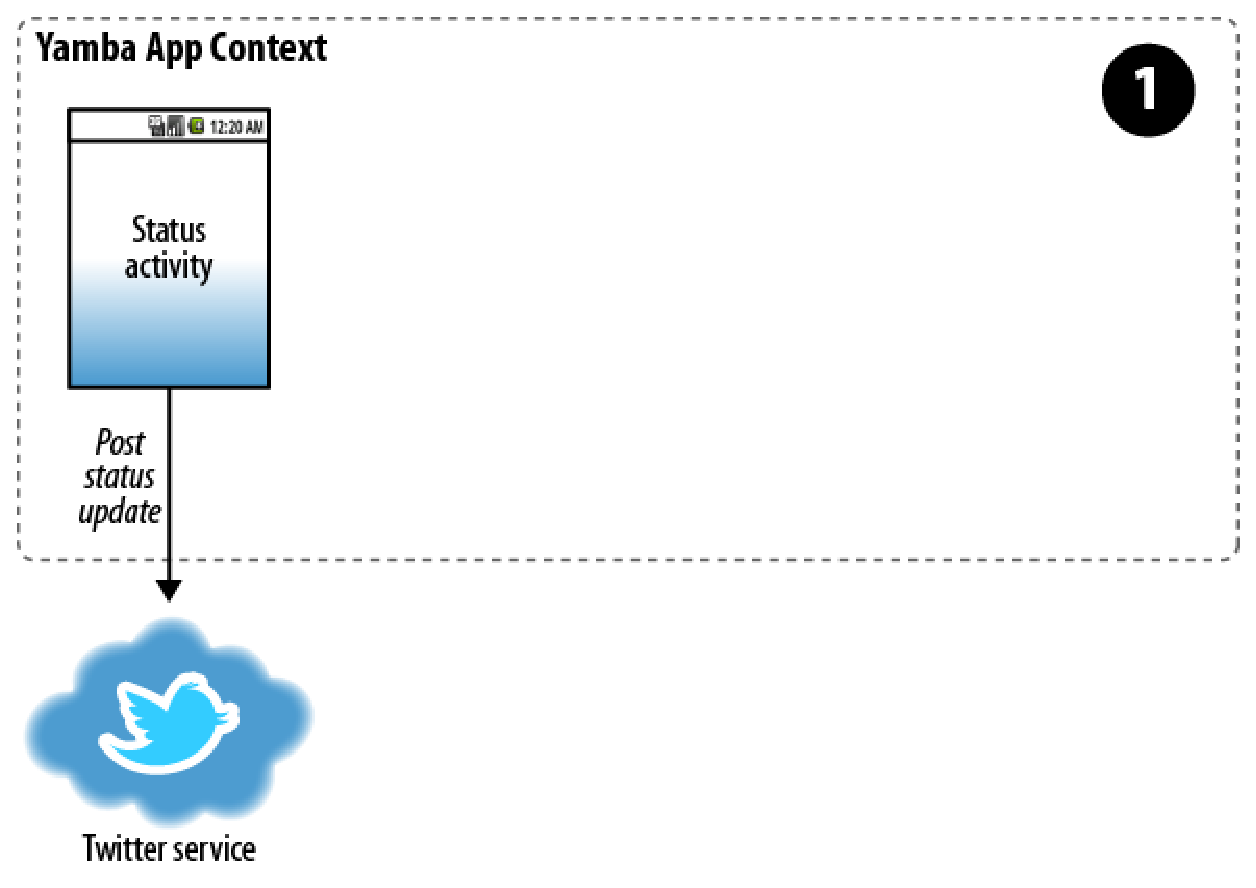
\includegraphics[width=0.65 \textwidth]{fig-64.eps}
\end{frame}
%------------------------------------------------------------------------------
\begin{frame}[fragile]
\frametitle{Git}
Push an existing repository from the command line
\begin{enumerate}
\item \texttt{git remote add origin https://github.com/carmelocuenca/Yamba.git}
\item \texttt{git push -u origin master}
\end{enumerate}
\end{frame}
%------------------------------------------------------------------------------
\begin{frame}[fragile]
\frametitle{Git}
\begin{enumerate}
\item \texttt{git status}
\item \texttt{git commit -a -m ``Color and Graphics''}
\end{enumerate}

\end{frame}
%------------------------------------------------------------------------------



%------------------------------------------------------------------------------